\documentclass[11pt,twoside]{article}\makeatletter
\IfFileExists{xcolor.sty}%
  {\RequirePackage{xcolor}}%
  {\RequirePackage{color}}
\usepackage{colortbl}

\IfFileExists{utf8x.def}%
 {\usepackage[utf8x]{inputenc}
    \PrerenderUnicode{–}
  }%
 {\usepackage[utf8]{inputenc}}
\usepackage[english]{babel}
\usepackage[T1]{fontenc}
\usepackage{float}
\usepackage[]{ucs}
\uc@dclc{8421}{default}{\textbackslash }
\uc@dclc{10100}{default}{\{}
\uc@dclc{10101}{default}{\}}
\uc@dclc{8491}{default}{\AA{}}
\uc@dclc{8239}{default}{\,}
\uc@dclc{20154}{default}{ }
\uc@dclc{10148}{default}{>}
\def\textschwa{\rotatebox{-90}{e}}
\def\textJapanese{}
\def\textChinese{}

\DeclareTextSymbol{\textpi}{OML}{25}
\usepackage{relsize}
\def\textsubscript#1{%
  \@textsubscript{\selectfont#1}}
\def\@textsubscript#1{%
  {\m@th\ensuremath{_{\mbox{\fontsize\sf@size\z@#1}}}}}
\def\textquoted#1{‘#1’}
\def\textsmall#1{{\small #1}}
\def\textlarge#1{{\large #1}}
\def\textoverbar#1{\ensuremath{\overline{#1}}}
\def\textgothic#1{{\fontspec{Lucida Blackletter}#1}}
\def\textcal#1{{\fontspec{Lucida Calligraphy}#1}}
\newenvironment{biblfree}{}{\ifvmode\par\fi }
\newenvironment{docImprint}{\vskip 6pt}{\ifvmode\par\fi }
\newenvironment{docDate}{}{\ifvmode\par\fi }
\newenvironment{docAuthor}{\ifvmode\vskip4pt\fontsize{16pt}{18pt}\selectfont\fi\itshape}{\ifvmode\par\fi }
\newenvironment{docTitle}{\vskip6pt\bfseries\fontsize{18pt}{22pt}\selectfont}{\par }
\newenvironment{titlePart}{}{\par }
\newenvironment{byline}{\vskip6pt\itshape\fontsize{16pt}{18pt}\selectfont}{\par }
\newenvironment{citbibl}{}{\ifvmode\par\fi }
\newenvironment{bibl}{}{}
\newenvironment{rubric}{}{}
\newenvironment{msItem}{\vskip 6pt}{\par}
\newenvironment{msHead}{\vskip 6pt}{\par}
\def\titlem#1{\emph{#1}}
\def\corr#1{#1}
\def\sic#1{#1}
\def\reg#1{#1}
\def\orig#1{#1}
\def\gap{}
\def\abbr#1{#1}
\def\expan#1{#1}
\RequirePackage{array}
\def\@testpach{\@chclass
 \ifnum \@lastchclass=6 \@ne \@chnum \@ne \else
  \ifnum \@lastchclass=7 5 \else
   \ifnum \@lastchclass=8 \tw@ \else
    \ifnum \@lastchclass=9 \thr@@
   \else \z@
   \ifnum \@lastchclass = 10 \else
   \edef\@nextchar{\expandafter\string\@nextchar}%
   \@chnum
   \if \@nextchar c\z@ \else
    \if \@nextchar l\@ne \else
     \if \@nextchar r\tw@ \else
   \z@ \@chclass
   \if\@nextchar |\@ne \else
    \if \@nextchar !6 \else
     \if \@nextchar @7 \else
      \if \@nextchar (8 \else
       \if \@nextchar )9 \else
  10
  \@chnum
  \if \@nextchar m\thr@@\else
   \if \@nextchar p4 \else
    \if \@nextchar b5 \else
   \z@ \@chclass \z@ \@preamerr \z@ \fi \fi \fi \fi
   \fi \fi  \fi  \fi  \fi  \fi  \fi \fi \fi \fi \fi \fi}

\gdef\arraybackslash{\let\\=\@arraycr}
\def\textxi{\ensuremath{\xi}}
\def\Panel#1#2#3#4{\multicolumn{#3}{){\columncolor{#2}}#4}{#1}}

\newcolumntype{L}[1]{){\raggedright\arraybackslash}p{#1}}
\newcolumntype{C}[1]{){\centering\arraybackslash}p{#1}}
\newcolumntype{R}[1]{){\raggedleft\arraybackslash}p{#1}}
\newcolumntype{P}[1]{){\arraybackslash}p{#1}}
\newcolumntype{B}[1]{){\arraybackslash}b{#1}}
\newcolumntype{M}[1]{){\arraybackslash}m{#1}}
\definecolor{label}{gray}{0.75}
\def\unusedattribute#1{\sout{\textcolor{label}{#1}}}
\DeclareRobustCommand*{\xref}{\hyper@normalise\xref@}
\def\xref@#1#2{\hyper@linkurl{#2}{#1}}
\begingroup
\catcode`\_=\active
\gdef_#1{\ensuremath{\sb{\mathrm{#1}}}}
\endgroup
\mathcode`\_=\string"8000
\catcode`\_=12\relax

\usepackage[a4paper,twoside,lmargin=1in,rmargin=1in,tmargin=1in,bmargin=1in]{geometry}
\usepackage{framed}

\definecolor{shadecolor}{gray}{0.95}
\usepackage{longtable}
\usepackage[normalem]{ulem}
\usepackage{fancyvrb}
\usepackage{fancyhdr}
\usepackage{marginnote}
\renewcommand*{\marginfont}{\itshape\footnotesize}
\setlength\marginparwidth{.75in}
\usepackage{graphicx}

\def\Gin@extensions{.pdf,.png,.jpg,.mps,.tif}

\IfFileExists{tipa.sty}{\usepackage{tipa}}{}
\usepackage{times}

  \pagestyle{fancy} 

\usepackage[pdftitle={A Christmas Carol},
 pdfauthor={Dickens, Charles, 1812-1870}]{hyperref}
\hyperbaseurl{}

	 \paperwidth210mm
	 \paperheight297mm
              
\def\@pnumwidth{1.55em}
\def\@tocrmarg {2.55em}
\def\@dotsep{4.5}
\setcounter{tocdepth}{3}
\clubpenalty=8000
\emergencystretch 3em
\hbadness=4000
\hyphenpenalty=400
\pretolerance=750
\tolerance=2000
\vbadness=4000
\widowpenalty=10000

\renewcommand\section{\@startsection {section}{1}{\z@}%
     {-1.75ex \@plus -0.5ex \@minus -.2ex}%
     {0.5ex \@plus .2ex}%
     {\reset@font\Large\bfseries\sffamily}}
\renewcommand\subsection{\@startsection{subsection}{2}{\z@}%
     {-1.75ex\@plus -0.5ex \@minus- .2ex}%
     {0.5ex \@plus .2ex}%
     {\reset@font\Large\sffamily}}
\renewcommand\subsubsection{\@startsection{subsubsection}{3}{\z@}%
     {-1.5ex\@plus -0.35ex \@minus -.2ex}%
     {0.5ex \@plus .2ex}%
     {\reset@font\large\sffamily}}
\renewcommand\paragraph{\@startsection{paragraph}{4}{\z@}%
     {-1ex \@plus-0.35ex \@minus -0.2ex}%
     {0.5ex \@plus .2ex}%
     {\reset@font\normalsize\sffamily}}
\renewcommand\subparagraph{\@startsection{subparagraph}{5}{\parindent}%
     {1.5ex \@plus1ex \@minus .2ex}%
     {-1em}%
     {\reset@font\normalsize\bfseries}}


\def\l@section#1#2{\addpenalty{\@secpenalty} \addvspace{1.0em plus 1pt}
 \@tempdima 1.5em \begingroup
 \parindent \z@ \rightskip \@pnumwidth 
 \parfillskip -\@pnumwidth 
 \bfseries \leavevmode #1\hfil \hbox to\@pnumwidth{\hss #2}\par
 \endgroup}
\def\l@subsection{\@dottedtocline{2}{1.5em}{2.3em}}
\def\l@subsubsection{\@dottedtocline{3}{3.8em}{3.2em}}
\def\l@paragraph{\@dottedtocline{4}{7.0em}{4.1em}}
\def\l@subparagraph{\@dottedtocline{5}{10em}{5em}}
\@ifundefined{c@section}{\newcounter{section}}{}
\@ifundefined{c@chapter}{\newcounter{chapter}}{}
\newif\if@mainmatter 
\@mainmattertrue
\def\chaptername{Chapter}
\def\frontmatter{%
  \pagenumbering{roman}
  \def\thechapter{\@roman\c@chapter}
  \def\theHchapter{\roman{chapter}}
  \def\@chapapp{}%
}
\def\mainmatter{%
  \cleardoublepage
  \def\thechapter{\@arabic\c@chapter}
  \setcounter{chapter}{0}
  \setcounter{section}{0}
  \pagenumbering{arabic}
  \setcounter{secnumdepth}{6}
  \def\@chapapp{\chaptername}%
  \def\theHchapter{\arabic{chapter}}
}
\def\backmatter{%
  \cleardoublepage
  \setcounter{chapter}{0}
  \setcounter{section}{0}
  \setcounter{secnumdepth}{2}
  \def\@chapapp{\appendixname}%
  \def\thechapter{\@Alph\c@chapter}
  \def\theHchapter{\Alph{chapter}}
  \appendix
}
\newenvironment{bibitemlist}[1]{%
   \list{\@biblabel{\@arabic\c@enumiv}}%
       {\settowidth\labelwidth{\@biblabel{#1}}%
        \leftmargin\labelwidth
        \advance\leftmargin\labelsep
        \@openbib@code
        \usecounter{enumiv}%
        \let\p@enumiv\@empty
        \renewcommand\theenumiv{\@arabic\c@enumiv}%
	}%
  \sloppy
  \clubpenalty4000
  \@clubpenalty \clubpenalty
  \widowpenalty4000%
  \sfcode`\.\@m}%
  {\def\@noitemerr
    {\@latex@warning{Empty `bibitemlist' environment}}%
    \endlist}

\def\tableofcontents{\section*{\contentsname}\@starttoc{toc}}
\parskip0pt
\parindent1em
\def\Panel#1#2#3#4{\multicolumn{#3}{){\columncolor{#2}}#4}{#1}}
\newenvironment{reflist}{%
  \begin{raggedright}\begin{list}{}
  {%
   \setlength{\topsep}{0pt}%
   \setlength{\rightmargin}{0.25in}%
   \setlength{\itemsep}{0pt}%
   \setlength{\itemindent}{0pt}%
   \setlength{\parskip}{0pt}%
   \setlength{\parsep}{2pt}%
   \def\makelabel##1{\itshape ##1}}%
  }
  {\end{list}\end{raggedright}}
\newenvironment{sansreflist}{%
  \begin{raggedright}\begin{list}{}
  {%
   \setlength{\topsep}{0pt}%
   \setlength{\rightmargin}{0.25in}%
   \setlength{\itemindent}{0pt}%
   \setlength{\parskip}{0pt}%
   \setlength{\itemsep}{0pt}%
   \setlength{\parsep}{2pt}%
   \def\makelabel##1{\upshape\sffamily ##1}}%
  }
  {\end{list}\end{raggedright}}
\newenvironment{specHead}[2]%
 {\vspace{20pt}\hrule\vspace{10pt}%
  \hypertarget{#1}{}%
  \markright{#2}%

  \pdfbookmark[2]{#2}{#1}%
  \hspace{-0.75in}{\bfseries\fontsize{16pt}{18pt}\selectfont#2}%
  }{}
      \def\TheFullDate{1970-01-01}
\def\TheID{\makeatother }
\def\TheDate{1970-01-01}
\title{A Christmas Carol}
\author{Dickens, Charles, 1812-1870}\makeatletter 
\makeatletter
\thispagestyle{empty}
\markright{\@title}\markboth{\@title}{\@author}
\renewcommand\small{\@setfontsize\small{9pt}{11pt}\abovedisplayskip 8.5\p@ plus3\p@ minus4\p@
\belowdisplayskip \abovedisplayskip
\abovedisplayshortskip \z@ plus2\p@
\belowdisplayshortskip 4\p@ plus2\p@ minus2\p@
\def\@listi{\leftmargin\leftmargini
               \topsep 2\p@ plus1\p@ minus1\p@
               \parsep 2\p@ plus\p@ minus\p@
               \itemsep 1pt}
}
\makeatother
\fvset{frame=single,numberblanklines=false,xleftmargin=5mm,xrightmargin=5mm}
\fancyhf{} 
\setlength{\headheight}{14pt}
\fancyhead[LE]{\bfseries\leftmark} 
\fancyhead[RO]{\bfseries\rightmark} 
\fancyfoot[RO]{}
\fancyfoot[CO]{\thepage}
\fancyfoot[LO]{\TheID}
\fancyfoot[LE]{}
\fancyfoot[CE]{\thepage}
\fancyfoot[RE]{\TheID}
\hypersetup{linkbordercolor=0.75 0.75 0.75,urlbordercolor=0.75 0.75 0.75,bookmarksnumbered=true}
\fancypagestyle{plain}{\fancyhead{}\renewcommand{\headrulewidth}{0pt}}\makeatother 
\begin{document}
\let\tabcellsep& \frontmatter 
\section*{(half title note)}\par
The Original Edition of A CHRISTMAS CAROL has been out of print for many years, and this Edition is a reprint from the stereotype plates of that Edition.
  \begin{titlepage}
  \begin{docTitle} \begin{titlePart}A Christmas carol. in prose. \end{titlePart} \begin{titlePart}being \textit{A Ghost Story of Christmas}\end{titlePart} \end{docTitle} \begin{byline}by \docAuthor{Charles Dickens.}\end{byline} \begin{byline}With illustrations by John Leech\end{byline} \begin{docImprint}London: Chapman and Hall, Ltd. 1893.\end{docImprint}
  \end{titlepage}
  \cleardoublepage

\section*{PREFACE }\par
I have endeavoured in this Ghostly little book, to raise the Ghost of an Idea, which shall not put my readers out of humour with themselves, with each other, with the season, or with me. May it haunt their houses pleasantly, and no one wish to lay it. 
\begin{quote}
Their faithful Friend and Servant, C.D. December, 1843.\end{quote}

\section*{Contents.}\begin{description}

\item[Stave I]Marley's ghost \hyperlink{S1}{1}
\item[Stave II]The first of the three spirits 
\item[Stave III ]The second of the three spirits 
\item[Stave IV ]The last of the spirits 
\item[Stave V]The end of it 
\end{description} \mainmatter 
\section*{(Bits of) A CHRISTMAS CAROL, and other things}
\section[Simple rendition tests]{Simple rendition tests}\par
‘Who-e debel you?’ — he at last said — ‘you no speak-e, damme, I kill-e.’ And so saying, the lighted tomahawk began flourishing about me in the dark.\par
‘Who-e debel you?’ — he at last said — ‘you no speak-e, damme, I kill-e.’ And so saying, the lighted tomahawk began flourishing about me in the dark. \par 
\begin{longtable}{P{0.20534262485482\textwidth}P{0.64465737514518\textwidth}}
\hline \rowcolor{label}Effect\tabcellsep Example\\\hline 
hi\tabcellsep This is hi rend="special" tag\\
emph\tabcellsep This is \textit{emph} tag\\
hi\tabcellsep This is \textit{hi} tag\\
typewriter\tabcellsep This is \texttt{typewriter} effect\\
bold\tabcellsep This is \textbf{bold} effect\\
normalweight\tabcellsep This is normalweight effect\\
smallcaps\tabcellsep This is \textsc{smallcaps} effect\\
capsall\tabcellsep This is \uppercase{capsall} effect\\
strikethrough\tabcellsep This is \sout{strikethrough} effect\\
strikedoublethrough\tabcellsep This is strikedoublethrough effect\\
color(red)\tabcellsep This is \textcolor{red}{color(red)} effect\\
underline\tabcellsep This is \uline{underline} effect\\
underwavyline\tabcellsep This is \uwave{underwavyline} effect\\
underdoubleline\tabcellsep This is \uuline{underdoubleline} effect\\
subscript\tabcellsep This is \textsubscript{subscript} effect\\
superscript\tabcellsep This is \textsuperscript{superscript} effect\\
bold italic red, done separately\tabcellsep \textbf{\textit{\textcolor{red}{rend test 1}}}\\
bold italic smallcaps\tabcellsep rend test 1 \footnote{Cairns 2003: 11. My work is Muellner 1996.}\end{longtable} \par
 
\section[Quotations]{Quotations}\par
A paragraph with a footnote containing a block-level object\footnote{We start with a quotation:
\leftline{This is the way the world ends}
\leftline{This is the way the world ends}
\leftline{This is the way the world ends}
\leftline{Not with a bang but a whimper.} which is from TS Eliot's \textit{Hollow men}}\par
Consider quotations: ‘This is a quote which is run on within the text and will have quote marks of some kind around it.’\par
Another quotation: \begin{quote}This is a block quote set off as such from the rest of the text\end{quote}\par
Here, by contrast is an ‘inline quotation’. Another strange thing about quotes is this: \begin{quote}You can put line breaks{\hskip1pt}\newline to determine where the line breaks{\hskip1pt}\newline Inside a block!\end{quote}
\section[Use of xml:lang]{Use of xml:lang}\par
He used a French \textit{radiateur}.\par
Languages: \textit{Deutsch}; \textit{Italiano}; \textit{Español}; \textit{Français}; \textit{Portugues}; \textit{Russian}; \textit{Svenska}; \textit{日本語}; \textit{中文}.
\section[del, gap, add, unclear etc]{del, gap, add, unclear etc}\par
[...]\gap{}. The \textsuperscript{interest} \& — affor [...]\gap{} the amount \textbf{over}{\hskip1pt}\newline  so small the interest afforded compared with cash, [...]\gap{} by the Annuity{\hskip1pt}\newline  note paper to those who \textbf{tutor} \textbf{think} it, or keep it, with a view {\hskip1pt}\newline  to circulation, will, when compared with cash be it ever so small be {\hskip1pt}\newline  so much \uline{profit}: compared with a the preceding higher {\hskip1pt}\newline  rate of interest, the reduced rate afforded by the Annuity {\hskip1pt}\newline  note paper, to those who, \textbf{tutor} if they \textbf{tutor} it, {\hskip1pt}\newline  will, have to depend upon to the extent of their {\hskip1pt}\newline  respective capitals so invested, have nothing else {\hskip1pt}\newline  to depend upon for their respective incomes, will, [...]\gap{} by the {\hskip1pt}\newline  amount of the difference, \textbf{foremost} itself as so {\hskip1pt}\newline  much less.
\section[Drama]{Drama} \begin{description} \item[Roderigo] 

Where shall we meet i' the morning?\end{description}
 \begin{description} \item[Iago] 

At my lodging.\end{description}
 \begin{description} \item[Roderigo] 

I'll be with thee betimes.\end{description}
 \begin{description} \item[Iago] 

Go to; farewell. Do you hear, Roderigo?\end{description}
 \begin{description} \item[Roderigo] 

What say you?\end{description}
 \begin{description} \item[Iago] 

No more of drowning, do you hear?\end{description}
 \begin{description} \item[Roderigo] 

I am changed: I'll go sell all my land.\end{description}

\section[Footnotes]{Footnotes}
\subsection[1 Zur Entstehung der Philosophischen  	UntersuchungenZu Textauszeichnungen und  	Siglen siehe die Legende.]{1 Zur Entstehung der Philosophischen Untersuchungen\footnote{Zu Textauszeichnungen und Siglen siehe die Legende.}}\par
Iriure dolor in hendrerit in vulputate velit esse molestie consequat, vel illum dolore eu feugiat nulla facilisis at vero eros et accumsan et iusto odio dignissim qui blandit praesent luptatum zzril delenit augue duis dolore te feugait nulla facilisi. Lorem ipsum dolor sit amet, consectetuer adipiscing elit, sed diam nonummy nibh euismod \footnote{Zu Textauszeichnungen und Siglen siehe die Legende.} Iriure dolor in hendrerit in vulputate velit esse molestie consequat, vel illum dolore eu feugiat nulla facilisis at vero eros et accumsan et iusto odio dignissim qui blandit praesent luptatum zzril delenit augue duis dolore te feugait nulla facilisi. Lorem ipsum dolor sit amet, consectetuer adipiscing elit, sed diam nonummy nibh euismod
\section[emph and links]{emph and links}\par
The \texttt{<emph>} element is used for linguistic emph\textit{asis}. ‘highlighting’ (\texttt{<soCalled>}) nor with \emph{shouting} (\texttt{<mentioned>}), \emph{transmogrification}, (a technical \texttt{<term>}), for which the \texttt{<gloss>} tag might be used to supply  \textit{a technical definition}).\par
Now for some links! We will start by cross-referring to a later section.\par
Here is a simple \texttt{<ptr>} to it: \textit{\hyperref[P1]{9. Lists}}. Here is a simple \texttt{<ref>}, a \hyperlink{P1}{reference to it}.\par
An \xref{http://www.bbc.co.uk}{external link} as ref and as ptr: \url{http://www.bbc.co.uk}.
\section[Tables]{Tables}\par
Tables may have cells that span multiple columns and rows. \par 
\begin{longtable}{P{0.5250764525993884\textwidth}P{0.23394495412844038\textwidth}P{0.09097859327217125\textwidth}}
 \hline\endfoot\hline\endlastfoot \endfirsthead \multicolumn{3}{c}{Pictures from Fagaras mountains(cont.)}\\\hline \endhead \caption{Pictures from Fagaras mountains}\\ \hline \rowcolor{label}Image\tabcellsep Description\tabcellsep Camera direction\\\hline 
SVG, JPEG, GIF or PNG format\\
\Panel{\textit{All pictures were taken on Jun 27, 2007 }}{label}{2}{l}\\
\noindent
\includegraphics[]{nature1.jpg}\tabcellsep Mountain flowers. \tabcellsep north\\
\noindent
\includegraphics[]{nature2.jpg}\tabcellsep Sunset over a secondary ridge.\tabcellsep north-east\\
\noindent
\includegraphics[]{nature3.jpg}\tabcellsep Glacier lake at 2100m altitude.\tabcellsep east\end{longtable} \par
  \par 
\begin{longtable}{P{0.3216216216216216\textwidth}P{0.13209459459459458\textwidth}P{0.2125\textwidth}P{0.1722972972972973\textwidth}P{0.011486486486486487\textwidth}}
 \hline\endfoot\hline\endlastfoot \endfirsthead \multicolumn{3}{c}{
            TEI Span Sample
          (cont.)}\\\hline \endhead \caption{
            TEI Span Sample
          }\\ \hline \rowcolor{label}\multicolumn{2}{){\columncolor{label}}l}{Spans \textbf{Horizontally}}\tabcellsep Header 3\tabcellsep \multicolumn{2}{){\columncolor{label}}l}{Spans \textbf{Horizontally}}\\\hline 
Spans \textbf{Vertically}\tabcellsep a\tabcellsep b\tabcellsep c\tabcellsep d\\
e\tabcellsep \multicolumn{2}{l}{Spans \textbf{both}}\tabcellsep f\\
g\tabcellsep g\\
i\tabcellsep j\tabcellsep \multicolumn{2}{l}{Spans \textbf{Horizontally}}\\
k\tabcellsep l\tabcellsep m\tabcellsep n\tabcellsep o\end{longtable} \par
 
\section[Lists]{Lists}\label{P1}\par
Various sorts of list are legal within paragraphs, and you can reference \hyperlink{birds}{items in lists}... \begin{enumerate}

\item Dogs
\item Zebras
\item \hypertarget{birds}{}Birds
\item Cats
\end{enumerate}\begin{description}

\item[100]first item 
\item[200]second item 
\item[300]third item 
\end{description} \par
The preceding lists was between paragraphs.\par
\leftline{\textbf{This untyped list has a heading and a nested glosslist }} \begin{itemize}

\item first item 
\item \begin{description}

\item[25]first item 
\item[35]second item 
\item[45]third item 
\end{description} 
\item third item 
\end{itemize} 
\section[Pictures]{Pictures} \par 
\begin{longtable}{P{0.1980173482032218\textwidth}P{0.6519826517967782\textwidth}}
\tabcellsep \noindent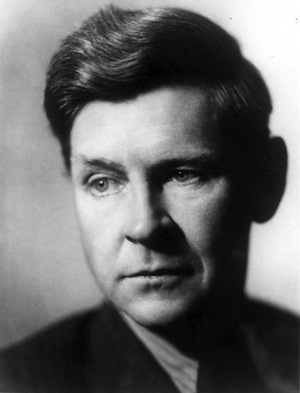
\includegraphics[]{portrait.jpg}\\
width="2.5in" \tabcellsep \noindent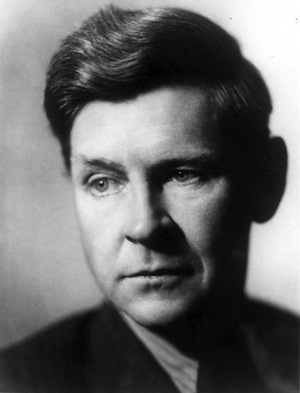
\includegraphics[width=2.5in,]{portrait.jpg}\\
width=".5in" \tabcellsep \noindent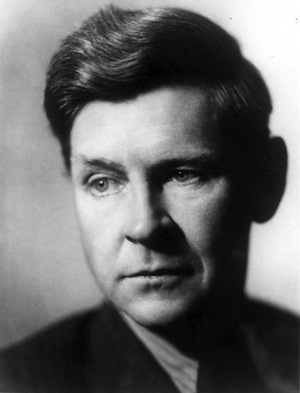
\includegraphics[width=0.5in,]{portrait.jpg}\\
scale=".5"\tabcellsep \noindent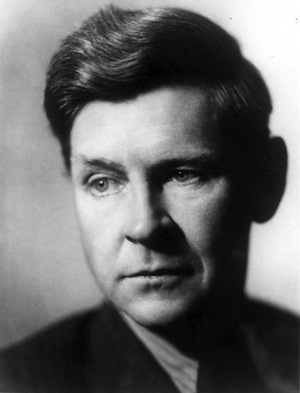
\includegraphics[scale=.5,]{portrait.jpg}\\
width="1in"\tabcellsep \noindent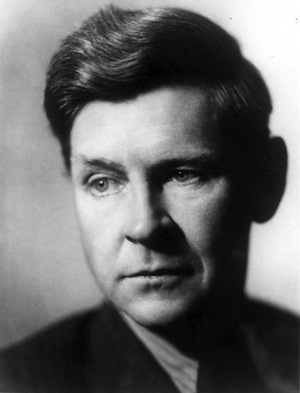
\includegraphics[width=1in,]{portrait.jpg}\\
width="1in" style="border:solid green 2pt"\tabcellsep \noindent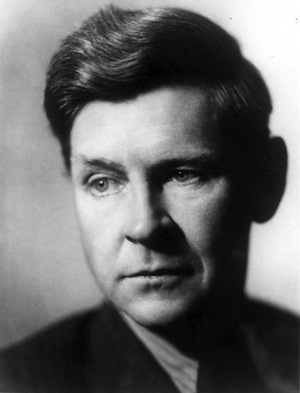
\includegraphics[width=1in,]{portrait.jpg}\\
height="1in"\tabcellsep \noindent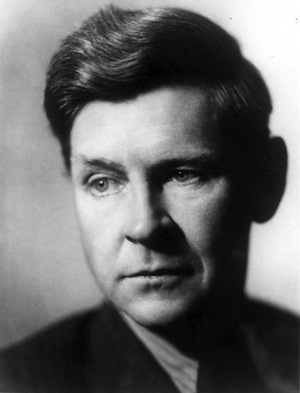
\includegraphics[height=1in,]{portrait.jpg}\\
height="1in" width="2in"\tabcellsep \noindent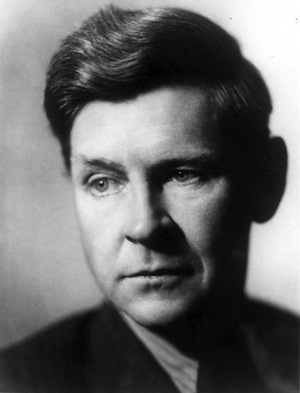
\includegraphics[width=2in,height=1in,]{portrait.jpg}\\
height="2in" width="1in"\tabcellsep \noindent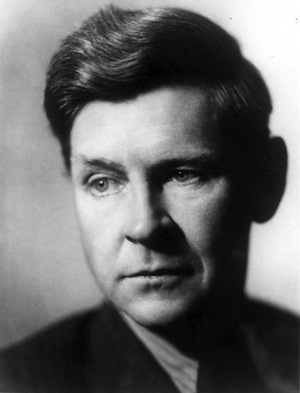
\includegraphics[width=1in,height=2in,]{portrait.jpg}\\
width="10\%"\tabcellsep \noindent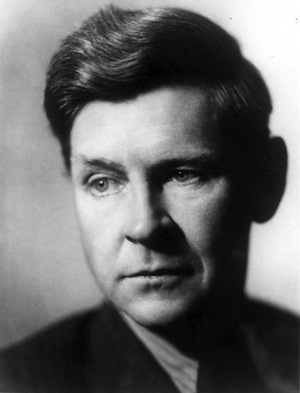
\includegraphics[width=0.1\textwidth,]{portrait.jpg}\\
height="10\%" width="10\%"\tabcellsep \noindent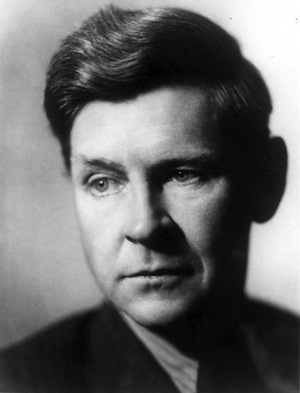
\includegraphics[width=0.1\textwidth,height=0.1\textheight,]{portrait.jpg}\end{longtable} \par
 
\section[MS catalogue]{MS catalogue}
\section{Identification}
where is it, repository name, identifier
\section[Extended prose: MARLEY'S GHOST]{Extended prose: MARLEY'S GHOST}\label{S1}% image:bar.jpg
\par
Marley was dead: to begin with. There is no doubt whatever about that. The register of his burial was signed by the clergyman, the clerk, the undertaker, and the chief mourner. Scrooge signed it. And Scrooge's name was good upon 'Change, for anything he chose to put his hand to. Old Marley was as dead as a door-nail. \par
Mind! I don't mean to say that I know, of my own knowledge, what there is particularly dead about a door-nail. I might have been inclined, myself, to regard a coffin-nail as the deadest piece of ironmongery in the trade. But the wisdom of our ancestors is in the simile; and my unhallowed  hands shall not disturb it, or the Country's done for. You will therefore permit me to repeat, emphatically, that Marley was as dead as a door-nail.\par
Scrooge knew he was dead? Of course he did. How could it be otherwise? Scrooge and he were partners for I don't know how many years. Scrooge was his sole executor, his sole administrator, his sole assign, his sole residuary legatee, his sole friend, and sole mourner. And even Scrooge was not so dreadfully cut up by the sad event, but that he was an excellent man of business on the very day of the funeral, and solemnised it with an undoubted bargain. \par
The mention of Marley's funeral brings me back to the point I started from. There is no doubt that Marley was dead. This must be distinctly understood, or nothing wonderful can come of the story I am going to relate. If we were not perfectly convinced that Hamlet's Father died before the play began, there would be nothing more remarkable in his taking a stroll at night, in an easterly wind, upon his own ramparts, than there  would be in any other middle-aged gentleman rashly turning out after dark in a breezy spot — say Saint Paul's Churchyard for instance — literally to astonish his son's weak mind.\par
Scrooge never painted out Old Marley's name. There it stood, years afterwards, above the ware-house door: Scrooge and Marley. The firm was known as Scrooge and Marley. Sometimes people new to the business called Scrooge Scrooge, and sometimes Marley, but he answered to both names. It was all the same to him. \par
Oh! But he was a tight-fisted hand at the grindstone, Scrooge! a squeezing, wrenching, grasping, scraping, clutching, covetous old sinner! Hard and sharp as flint, from which no steel had ever struck out generous fire; secret, and self-contained, and solitary as an oyster. The cold within him froze his old features, nipped his pointed nose, shrivelled his cheek, stiffened his gait; made his eyes red, his thin lips blue; and spoke out shrewdly in his grating voice. A frosty rime was on his head, and on his eyebrows, and his wiry chin. He  carried his own low temperature always about with him; he iced his office in the dog-days; and didn't thaw it one degree at Christmas.\par
External heat and cold had little influence on Scrooge. No warmth could warm, no wintry weather chill him. No wind that blew was bitterer than he, no falling snow was more intent upon its purpose, no pelting rain less open to entreaty. Foul weather didn't know where to have him. The heaviest rain, and snow, and hail, and sleet, could boast of the advantage over him in only one respect. They often ‘came down’ handsomely, and Scrooge never did.\par
Nobody ever stopped him in the street to say, with gladsome looks, ‘My dear Scrooge, how are you. When will you come to see me.’ No beggars implored him to bestow a trifle, no children asked him what it was o'clock, no man or woman ever once in all his life inquired the way to such and such a place, of Scrooge. Even the blindmen's dogs appeared to know him; and when they saw him coming on, would tug their owners into doorways  and up courts; and then would wag their tails as though they said, ‘No eye at all is better than an evil eye, dark master! ’\par
But what did Scrooge care! It was the very thing he liked. To edge his way along the crowded paths of life, warning all human sympathy to keep its distance, was what the knowing ones call ‘nuts’ to Scrooge.\par
Once upon a time — of all the good days in the year, on Christmas Eve — old Scrooge sat busy in his counting-house. It was cold, bleak, biting weather: foggy withal: and he could hear the people in the court outside, go wheezing up and down, beating their hands upon their breasts, and stamping their feet upon the pavement stones to warm them. The city clocks had only just gone three, but it was quite dark already: it had not been light all day: and candles were flaring in the windows of the neighbouring offices, like ruddy smears upon the palpable brown air. The fog came pouring in at every chink and keyhole, and was so dense without, that although the court was of the  narrowest, the houses opposite were mere phantoms. To see the dingy cloud come drooping down, obscuring everything, one might have thought that Nature lived hard by, and was brewing on a large scale.\par
The door of Scrooge's counting-house was open that he might keep his eye upon his clerk, who in a dismal little cell beyond, a sort of tank, was copying letters. Scrooge had a very small fire, but the clerk's fire was so very much smaller that it looked like one coal. But he couldn't replenish it, for Scrooge kept the coal-box in his own room; and so surely as the clerk came in with the shovel, the master predicted that it would be necessary for them to part. Wherefore the clerk put on his white comforter, and tried to warm himself at the candle; in which effort, not being a man of a strong imagination, he failed. \par
‘A merry Christmas, uncle! God save you!’ cried a cheerful voice. It was the voice of Scrooge's nephew, who came upon him so quickly that this was the first intimation he had of his approach. \par
‘Bah!’ said Scrooge, ‘Humbug!’\par
He had so heated himself with rapid walking in the fog and frost, this nephew of Scrooge's, that he was all in a glow; his face was ruddy and handsome; his eyes sparkled, and his breath smoked again. \par
‘Christmas a humbug, uncle!’ said Scrooge's nephew. ‘You don't mean that, I am sure.’\par
‘I do,’ said Scrooge. ‘Merry Christmas! What right have you to be merry? what reason have you to be merry? You're poor enough.’\par
‘Come, then,’ returned the nephew gaily. ‘What right have you to be dismal? what reason have you to be morose? You're rich enough.’\par
Scrooge having no better answer ready on the spur of the moment, said, ‘Bah!’ again; and followed it up with ‘Humbug.’\par
‘Don't be cross, uncle,’ said the nephew.\par
‘What else can I be,’ returned the uncle, ‘when I live in such a world of fools as this Merry Christmas! Out upon merry Christmas. What's Christmas time to you but a time for paying bills without money; a time for finding yourself a year older, but not an hour richer; a time for balancing your books and having every item in 'em through a round dozen of months presented dead against you? If I could work my will,’ said Scrooge indignantly, ‘every idiot who goes about with ‘Merry Christmas’ on his lips, should be boiled with his own pudding, and buried with a stake of holly through his heart. He should!’\par
‘Uncle!’ pleaded the nephew.\par
‘Nephew!’ returned the uncle, sternly, ‘keep Christmas in your own way, and let me keep it in mine.’\par
‘Keep it!’ repeated Scrooge's nephew. ‘But you don't keep it.’\par
‘Let me leave it alone, then,’ said Scrooge. ‘Much good may it do you! Much good it has ever done you!’\par
‘There are many things from which I might have derived good, by which I have not profited, I dare say,’ returned the nephew: ‘Christmas among the rest. But I am sure I have always thought of Christmas time, when it has come round — apart from the veneration due to its sacred name and origin, if anything belonging to it can be apart from that — as a good time: a kind, forgiving, charitable, pleasant time: the only time I know of, in the long calendar of the year, when men and women seem by one consent to open their shut-up hearts freely, and to think of people below them as if they really were fellow-passengers to the grave, and not another race of creatures bound on other journeys. And therefore, uncle, though it has never put a scrap of gold or silver in my pocket, I believe that it \textit{has} done me good, and \textit{will} do me good; and I say, God bless it!’\par
The clerk in the tank involuntarily applauded. Becoming immediately sensible of the impropriety, he poked the fire, and extinguished the last frail spark for ever. \par
‘Let me hear another sound from \textit{you},’ said Scrooge, ‘and you'll keep your Christmas by losing your situation. You're quite a powerful speaker, sir,’ he added, turning to his nephew. ‘I wonder you don't go into Parliament.’\par
‘Don't be angry, uncle. Come! Dine with us to-morrow.’\par
Scrooge said that he would see him — yes, indeed he did. He went the whole length of the expression, and said that he would see him in that extremity first. \par
‘But why?’ cried Scrooge's nephew. ‘Why?’\par
‘Why did you get married?’ said Scrooge.\par
‘Because I fell in love.’\par
‘Because you fell in love!’ growled Scrooge, as if that were the only one thing in the world more ridiculous than a merry Christmas. ‘Good afternoon!’\par
‘Nay, uncle, but you never came to see me before that happened. Why give it as a reason for not coming now?’\par
‘Good afternoon,’ said Scrooge.\par
‘I want nothing from you; I ask nothing of you; why cannot we be friends?’\par
‘Good afternoon,’ said Scrooge.\par
‘I am sorry, with all my heart, to find you so resolute. We have never had any quarrel, to which I have been a party. But I have made the trial in homage to Christmas, and I'll keep my Christmas humour to the last. So A Merry Christmas, uncle!’\par
‘Good afternoon!’ said Scrooge.\par
‘And A Happy New Year!’\par
‘Good afternoon!’ said Scrooge.\par
His nephew left the room without an angry word, notwithstanding. He stopped at the outer door to bestow the greeting of the season on the clerk, who, cold as he was, was warmer than Scrooge; for he returned them cordially. \par
‘There's another fellow,’ muttered Scrooge; who overheard him: ‘my clerk, with fifteen shillings a week, and a wife and family, talking about a merry Christmas. I'll retire to Bedlam.’\par
This lunatic, in letting Scrooge's nephew out, had let two other people in. They were portly gentlemen, pleasant to behold, and now stood, with their hats off, in Scrooge's office. They had books and papers in their hands, and bowed to him. \par
‘Scrooge and Marley's, I believe,’ said one of the gentlemen, referring to his list. ‘Have I the pleasure of addressing Mr Scrooge, or Mr Marley?’\par
‘Mr Marley has been dead these seven years,’ Scrooge replied. ‘He died seven years ago, this very night.’\par
‘We have no doubt his liberality is well represented by his surviving partner,’ said the gentleman, presenting his credentials.\par
It certainly was; for they had been two kindred spirits. At the ominous word ‘liberality’, Scrooge frowned, and shook his head, and handed the credentials back.\par
‘At this festive season of the year, Mr Scrooge,’ said the gentleman, taking up a pen, ‘it is more than usually desirable that we should make some slight provision for the Poor and destitute, who suffer greatly at the present time. Many thousands are in want of common necessaries; hundreds of thousands are in want of common comforts, sir.’\par
‘Are there no prisons?’ asked Scrooge.\par
‘Plenty of prisons,’ said the gentleman, laying down the pen again. \par
‘And the Union workhouses?’ demanded Scrooge. ‘Are they still in operation?’\par
‘They are. Still,’ returned the gentleman, ‘I wish I could say they were not.’\par
‘The Treadmill and the Poor Law are in full vigour, then?’ said Scrooge.\par
‘Both very busy, sir.’\par
‘Oh! I was afraid, from what you said at first, that something had occurred to stop them in their useful course,’ said Scrooge. ‘I'm very glad to hear it.’\par
‘Under the impression that they scarcely furnish Christian cheer of mind or body to the multitude,’ returned the gentleman, ‘a few of us are endeavouring to raise a fund to buy the Poor some meat and drink, and means of warmth. We choose this time, because it is a time, of all others, when Want is keenly felt, and Abundance rejoices. What shall I put you down for?’\par
‘Nothing!’ Scrooge replied.\par
‘You wish to be anonymous?’\par
‘I wish to be left alone,’ said Scrooge. ‘Since  you ask me what I wish, gentlemen, that is my answer. I don't make merry myself at Christmas and I can't afford to make idle people merry. I help to support the establishments I have mentioned: they cost enough: and those who are badly off must go there.’\par
‘Many can't go there; and many would rather die.’\par
‘If they would rather die,’ said Scrooge, ‘they had better do it, and decrease the surplus population. Besides — excuse me — I don't know that.’\par
‘But you might know it,’ observed the gentleman.\par
‘It's not my business,’ Scrooge returned. ‘It's enough for a man to understand his own business, and not to interfere with other people's. Mine occupies me constantly. Good afternoon, gentlemen!’\par
Seeing clearly that it would be useless to pursue their point, the gentlemen withdrew. Scrooge resumed his labours with an improved opinion of himself, and in a more facetious temper than was usual with him. \par
Foggier yet, and colder! Piercing, searching, biting cold. If the good Saint Dunstan had but nipped the Evil Spirit's nose with a touch of such weather as that,  {\small\itshape [Note: test of a note]}  instead of using his familiar weapons, then indeed he would have roared to lusty purpose. The owner of one scant young nose, gnawed and mumbled by the hungry cold as bones are gnawed by dogs, stooped down at Scrooge's keyhole to regale him with a Christmas carol: but at the first sound of 
\begin{quote}
\leftline{God bless you, merry gentleman! }
\leftline{May nothing you dismay! }\end{quote}
 Scrooge seized the ruler with such energy of action that the singer fled in terror, leaving the keyhole to the fog and even more congenial frost.
\section[Linking]{Linking}\par
\url{http://www.bbc.co.uk}\par
\url{https://staff.oucs.ox.ac.uk}\par
foo\par
\xref{http://www.example.com/personography.html\#fred}{Fred}\par
\xref{http://www.example.com/getBibl.xql?name=Jones&year=76}{Jones 76}
\section[Testing preservation of ID]{Testing preservation of ID}\par
Lorem ipsum dolor sit amet Lorem ipsum dolor sit amet. Lorem ipsum dolor sit amet Lorem ipsum dolor sit amet. Lorem ipsum dolor sit amet Lorem ipsum dolor sit amet. With references to \begin{itemize}

\item \hyperlink{thisQuotation}{Quotation}
\item \hyperlink{thisCitation}{Citation}
\item \hyperlink{thisParagraph}{Paragraph}
\item \hyperlink{thisReference}{Reference}
\item \hyperlink{movingAnchor}{Anchor}
\item \hyperlink{thisTitle}{Title}
\end{itemize} \par
I wonder what are the xml-ids preserved in a transformation to XHTML, in particular in the case of quotations. So, let’s try :
\begin{quote}
\par
Something longer. Lorem ipsum dolor sit amet Lorem ipsum dolor sit amet. Lorem ipsum dolor sit amet Lorem ipsum dolor sit amet.\par
\begin{biblfree}In \titlem{Somewhere}.\end{biblfree}
\end{quote}

\section[Choice, sic, corr, reg, orig]{Choice, sic, corr, reg, orig}\par
voro þav sammędd syskin in heilagri {\hskip1pt}\newline  olafr konvngr ok fyrnefnd [\corr{gvnnhilldr}].\par
Lastly, That, upon his solemn oath to observe all the above articles, the said man-mountain shall have a daily allowance of meat and drink sufficient for the support of [\corr{1728}] of our subjects, with free access to our royal person, and other marks of our \reg{favor}.
\section[Verbatim]{Verbatim}\par
an egXML in a list: \begin{itemize}

\item \par\bgroup\ttfamily\small\selectfont \begin{shaded}\noindent\mbox{}{<\textbf{div}\hspace*{6pt}{xml:id}="{test99}"\hspace*{6pt}{rend}="{whatever}">}\mbox{}\newline 
\hspace*{6pt}{<\textbf{head}>}Choice, sic, corr, reg, orig{</\textbf{head}>}\mbox{}\newline 
\hspace*{6pt}{<\textbf{p}>}v{<\textbf{ex}>}oro{</\textbf{ex}>} þav sam{<\textbf{ex}>}m{</\textbf{ex}>}ędd syskin in\mbox{}\newline 
\hspace*{6pt}\hspace*{6pt} hei{<\textbf{ex}>}lagr{</\textbf{ex}>}i {<\textbf{lb}/>} ol{<\textbf{ex}>}afr{</\textbf{ex}>} k{<\textbf{ex}>}onvng{</\textbf{ex}>}r\mbox{}\newline 
\hspace*{6pt}{<\textbf{ex}>}ok{</\textbf{ex}>} fyrnefnd\mbox{}\newline 
\hspace*{6pt}{<\textbf{choice}>}\mbox{}\newline 
\hspace*{6pt}\hspace*{6pt}\hspace*{6pt}{<\textbf{sic}>}gvn{<\textbf{ex}>}n{</\textbf{ex}>}hillde{</\textbf{sic}>}\mbox{}\newline 
\hspace*{6pt}\hspace*{6pt}\hspace*{6pt}{<\textbf{corr}>}gvn{<\textbf{ex}>}n{</\textbf{ex}>}hilldr{</\textbf{corr}>}\mbox{}\newline 
\hspace*{6pt}\hspace*{6pt}{</\textbf{choice}>}.{</\textbf{p}>}\mbox{}\newline 
{</\textbf{div}>}\end{shaded}\egroup\par 
\end{itemize} 
\end{document}
